\documentclass[10pt, compress]{beamer}

\usetheme{m}

\usepackage{booktabs}
\usepackage[scale=2]{ccicons}
\usepackage[outputdir=.texpadtmp]{minted}
\usepackage{FiraSans}
\usepackage{graphicx}
\usepackage{caption}
\usepackage{subcaption}

\usemintedstyle{trac}

\title{Lichtsteuerungsautomatisierung}
\subtitle{DAT Projekt}
\date{\today}
\author{Thiemann, Schuller, Wildt}
\institute{Hochschule Rosenheim}

\begin{document}

\maketitle

\section{Automatisierte Lichtsteuerung}

\plain{ }{
  \vspace{-2em}
  \begin{center}
    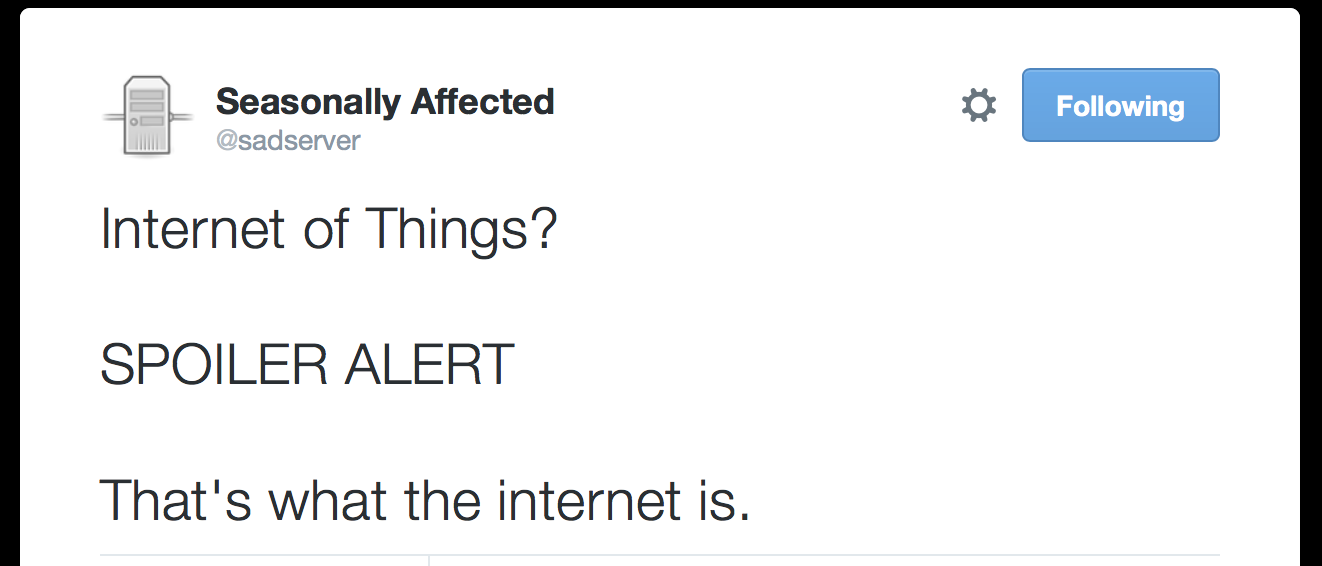
\includegraphics[width=0.9\textwidth]{images/sadserver1}
  \end{center}
}

\section{Internet of Things}

\section{Technologie}

\begin{frame}{Technologie - Idee}
  \begin{center}
    
\includegraphics[width=0.9\textwidth]{images/grobarchitektur}
  \end{center}
\end{frame}

\begin{frame}{Technologie - Fokus}
  \begin{center}
    
\includegraphics[width=0.9\textwidth]{images/realworld}
  \end{center}
\end{frame}

\section{Hardware}

\begin{frame}{Hardware}
  \begin{itemize}
    \item RaspberryPi 2
	\item RaspBee
	\item Philips Hue LED
  \end{itemize}
\end{frame}

\begin{frame}{Final}

  \begin{center}\huge Fragen?\end{center}
    
  \vspace{1cm}
  \begin{center}
  {\small

  The \LaTeX \ theme \emph{mtheme} is licensed under a
  \href{http://creativecommons.org/licenses/by-sa/4.0/}{Creative Commons
  Attribution-ShareAlike 4.0 International License}.}

  \ccbysa
  
  \end{center}

\end{frame}

\end{document}